For Neural Networks I have decided to use a convulutional neural network because of
it great performance in problems that can be represented as an "image". This because it
convolutional neural networks(CNN's) works by recognizing paterns in images or represented as
a matrix or tensor(multidimension matrix) in the computer. It does so by using convolutional,
pooling and voting layers. Multiple of these can be stacked to create a very a precise recongising
images.

\begin{figure}[H]
    \centering
        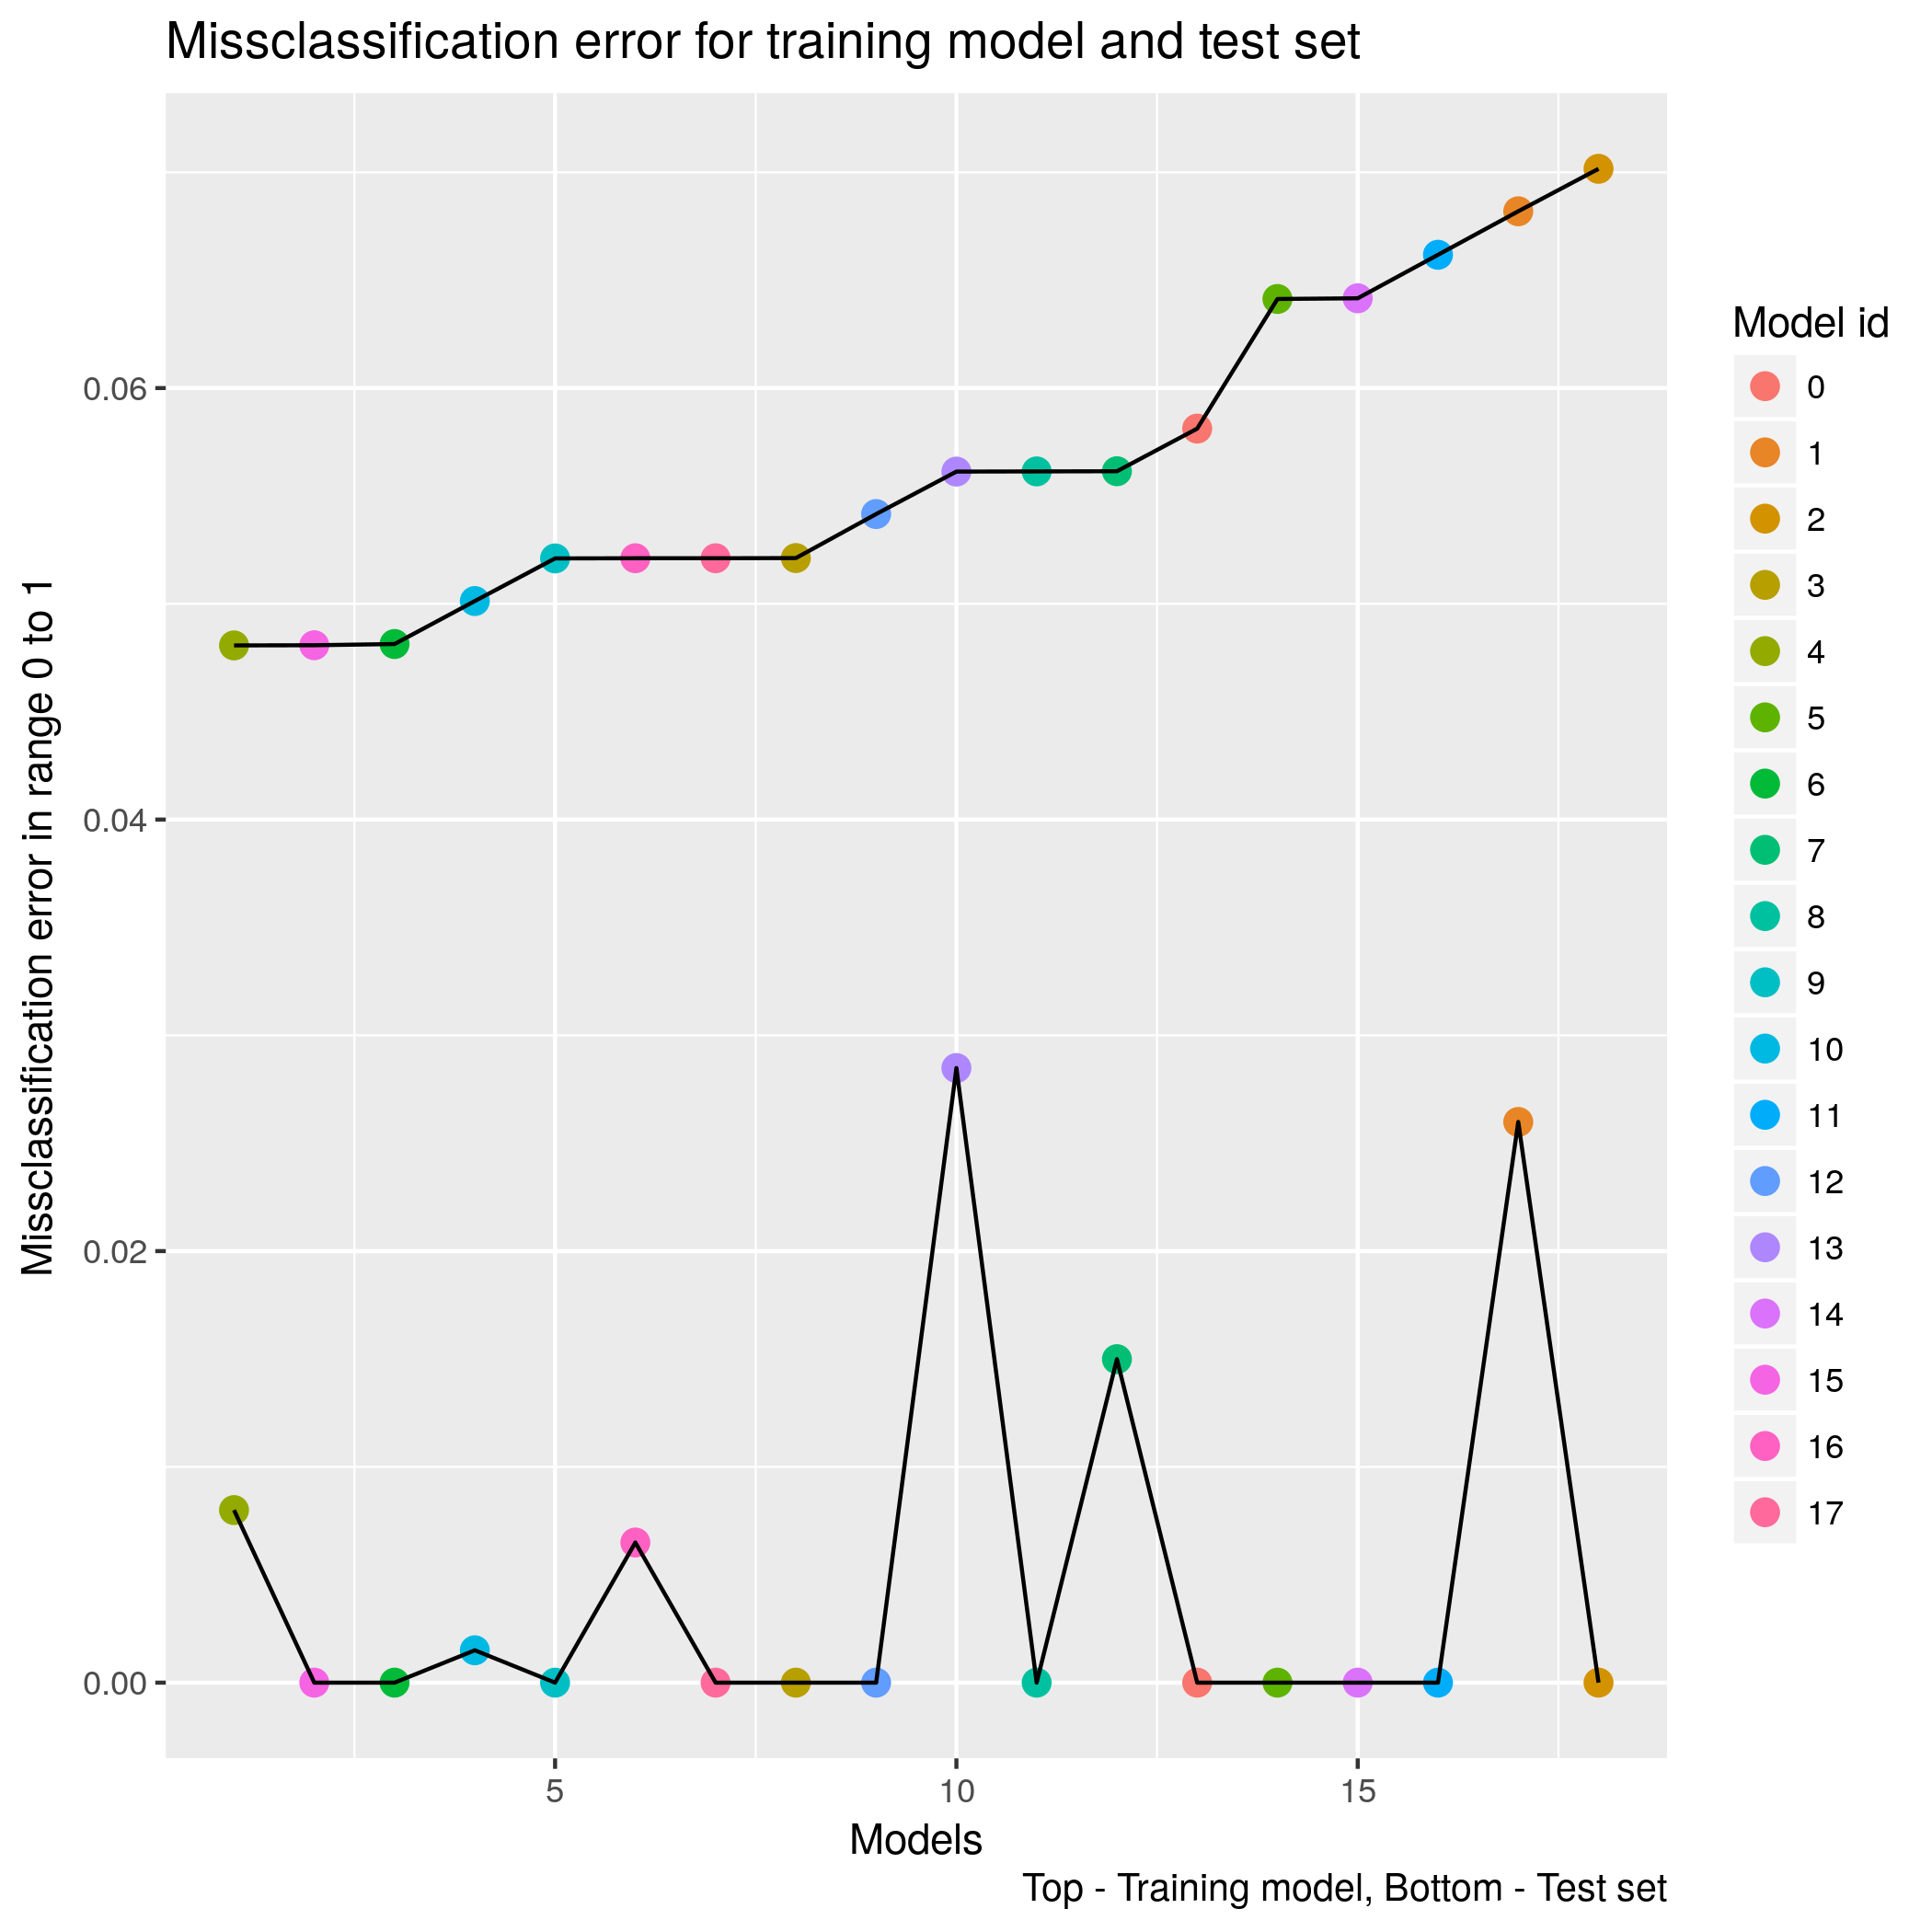
\includegraphics[width =.9\linewidth]{../R_scripts/Neural_Networks/results_NN/per_class_error.png}
    \caption{Error measures $E_{out}$ and $E_{val}$ are plotted for different sizes of training and validation sets.}
  \label{plot:1ii}
\end{figure}
